\chapter{Fundamentação}\label{ch:Fundamentacao}

A fundamentação teórica é um elemento crucial para a compreensão dos fundamentos teóricos que dão base aos conceitos que permeiam o objeto de estudo em uma determinada pesquisa. O capítulo de fundamentação surge então para munir o pesquisador dos conhecimentos necessários para o andamento e a conclusão de sua pesquisa. Ao mesmo tempo, a fundamentação auxilia outros pesquisadores na identificação das bases do conhecimento teórico que guiaram determinado estudo. 

O corrente estudo tem como cerne a validação de um programa educacional para a prevenção da violência sexual infantil baseado na dinâmica de jogos sérios. Deste modo, a \autoref{sec:JogosSerios} fundamenta o conceito de Jogos Sérios. A \autoref{sec:Engenharia} trás alguns conceitos sobre o desenvolvimento de jogos. A \autoref{sec:Avaliativos} discute sobre modelos voltados para a avaliação de programas educacionais na temática de prevenção a violência sexual infantil.


\section{Jogos Sérios}\label{sec:JogosSerios}

O termo \underline{Jo}g\underline{o Sério} (em inglês: \textit{Serious Game}) surge pela primeira vez na história em 1970 \cite{clark1970serious}. Desde então, o termo passou por inúmeras revisões até alcançar uma definição geral, a qual classifica como Jogo Sério: todos os jogos projetados para uma finalidade principal que não a pura diversão \cite{michael2005serious, de2015aprendizagem, laamarti2014overview}.

A definição geral de Jogos Sérios permite identificar que os jogos classificados como sérios antecedem a própria origem do termo. Isso pois, a história conta que antes da década de 70, alguns jogos já eram utilizados para outros propósitos além do entretenimento \cite{wilkinson2016brief}. Salienta-se, no entanto, que o termo não encontra-se verdadeiramente consolidado na literatura científica da área, existindo inclusive várias definições e termos correlatos \cite{pourabdollahian2012serious}.

Para definir melhor o termo \underline{Jo}g\underline{o Sério} que fundamentará e guiará o andamento do presente estudo, buscou-se separar o conceito e interpretar individualmente as palavras que o compõem. O termo \underline{Jo}g\underline{o} demarca o conjunto de atividades regidas por uma estrutura de regras focadas na diversão e no entretenimento \cite{kishimoto1994jogo}. Já o termo \underline{Sério} define um propósito prático a este conjunto de atividades, geralmente sendo pedagógico ou motor \cite{schroeder2017wobu, baptista2017jogos}. %(com os Exergames = Jogos Ativos). 
A Figura \ref{fig:JS}, ilustra de forma resumida os conceitos que fundamentam a definição de \underline{Jo}g\underline{o Sério} do atual trabalho.  

%Jogo: “é uma atividade mais estruturada e estabelecida por um princípio de regras mais explícitas” que integra tanto o objeto quanto a brincadeira (Kishimoto, 1994) ou “ação de jogar” (Bertoldo & others, 2000) %https://repositorio-aberto.up.pt/bitstream/10216/110820/2/253022.pdf

%Um game é uma atividade lúdica composta por uma série de ações e decisões, limitado por regras e pelo universo do game, que resultam em uma condição final. As regras e o universo do game são apresentados por meios eletrônicos e controlados por um programa digital (...) [e] existem para proporcionar uma estrutura e um contexto para as ações de um jogador. As regras também existem para criar situações interessantes com o objetivo de desafiar e se contrapor ao jogador. Jogos Sérios são aplicações que mesclam aspectos sérios como o ensino, a aprendizagem, a comunicação e a informação, com o lúdico e interativo fornecido pelos games, sendo o principal objetivo outro além do puro entretenimento. Criar um Jogo Sério é conseguir fundir de forma atraente e interessante informações para ensino, com interações dinâmicas e lúdicas (BOYLE; CONNOLLY; HAINEY, 2011, p. 71).%https://www.udesc.br/arquivos/cct/id_cpmenu/1024/diego_buchinger__1__15167055468902_1024.pdf

%Esta combinação tem como propósito tornar o conteúdoprático, útil (sério) e jogável, o que é alcançado por meio do desenvolvimento decenários que são ao mesmo tempo práticos e agradáveis.%https://webcache.googleusercontent.com/search?q=cache:fWC_TzjZ76QJ:https://www.br-ie.org/pub/index.php/pie/article/download/6595/4506+&cd=1&hl=pt-BR&ct=clnk&gl=br

%computer application, for which the original intention is to combine with consistency, both serious (Serious) aspects such as non-exhaustive and non-exclusive, teaching, learning, communication, or the information, with playful springs from the video game (Game). %http://hayka-kultura.org/images/Proceedings%20SGS%20Wkshp%202011%20ind%2004.pdf#page=11

\pagebreak

\begin{figure}[htb]

	\caption{\label{fig:JS}Infrográfico da terminologia Jogo Sério}\vspace{-0,5cm}
  \begin{center}
    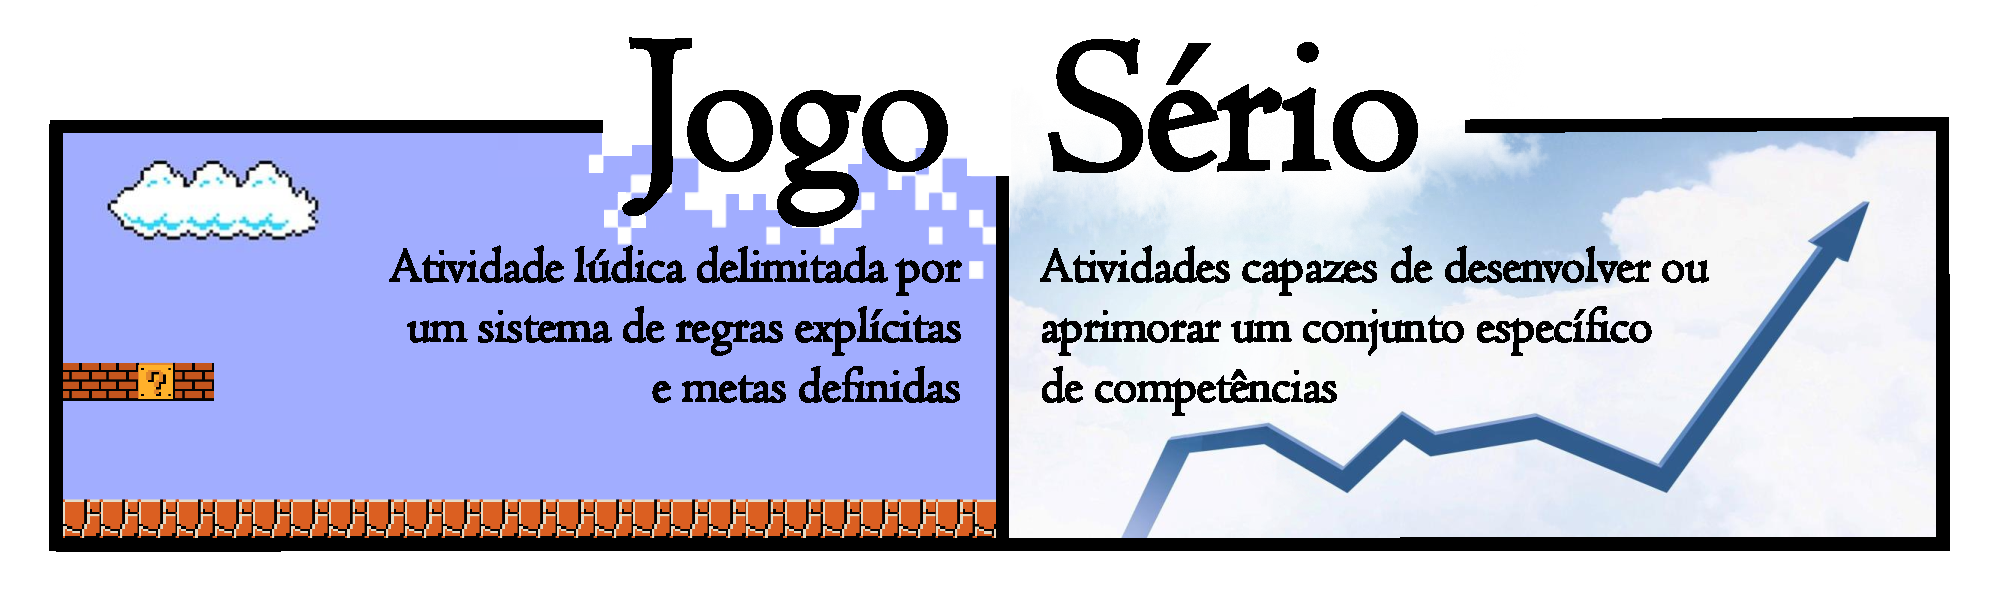
\includegraphics[width=\linewidth]{./Figuras/JogoSerio.pdf}
	\end{center} \vspace{-0,9cm}
  \legend{Fonte: os autores}

\end{figure}
%[GRAFICOOOOOO]http://downloads.hindawi.com/journals/ijcgt/2014/358152.pdf

\vspace{-0,4cm}

A Figura \ref{fig:JS} define separadamente a palavra \underline{Jo}g\underline{o} e \underline{Sério}. A união das definições dá o conceito de \underline{Jo}g\underline{o Sério} mais comum encontrado em pesquisas na área \cite{michael2005serious}. Enfatiza-se que para uma atividade se configurar como jogo, basta obedecer a um conjunto de regras e objetivos. Um jogo nessa definição não precisa de quaisquer outros artefatos para se configurar como tal, podendo ainda, ocorrer individualmente ou coletivamente. Para um jogo abranger o caráter \underline{Sério} é necessário que o mesmo trabalhe em algum nível as habilidades físicas ou intelectuais de seus jogadores. 

\vspace{-0,1cm}

O aprimoramento ou desenvolvimento de habilidades físicas normalmente é associado aos \underline{Jo}g\underline{os Ativos} \cite{araujo2017exergames, schroeder2017wobu}. Já o aprimoramento ou desenvolvimento de habilidades intelectuais é geralmente relacionado aos \underline{Jo}g\underline{os Educativos}. Pode-se dizer então que a classe de \underline{Jo}g\underline{o Sério} é uma generalização das áreas de \underline{Jo}g\underline{os Ativos} e \underline{Jo}g\underline{os Educativos}. Salienta-se, no entanto, que para um jogo ser classificado como sério, não se faz necessário que o jogo compreenda ambas as áreas. Todavia, na definição mais aceita, um jogo sério deve abranger a área dos  \underline{Jo}g\underline{os Di}g\underline{itais} \cite{laamarti2014overview}.

%Outra área também associada aos jogos sérios é a área dos \underline{Jo}g\underline{os Di}g\underline{itais}.

\vspace{-0,1cm}

Os \underline{Jo}g\underline{os Di}g\underline{itais} são todo o conjunto de jogos, os quais são jogáveis apenas por intermédio de mídias digitais \cite{lucchese2009conceituaccao}. Os jogos digitais, englobam a definição clássica de \underline{Jo}g\underline{o}, necessitando também de um conjunto de regras e objetivos, porém acrescidos de um motor de jogo e uma interface interativa \cite{battaiola2000jogos}. Enquanto o motor de jogo fica responsável por controlar o conjunto de regras que rege o jogo. A interface interativa se encarrega de converter o jogo em si para sinais visuais e sonoros compreensíveis ao jogador.

\vspace{-0,1cm}

Os jogos digitais possuem um sistema de regras mais rígido em relação aos jogos clássicos, devido ao contexto computacional do motor de jogo. O mesmo contexto computacional também é responsável por trazer maior segurança aos jogos digitais em relação aos clássicos, uma vez que a interface interativa é capaz de construir um ambiente lúdico inteiramente virtual, no qual os jogadores possam passar por situações de perigo sem que isso reflita em vias de fato em riscos aos jogadores \cite{lucchese2009conceituaccao}.

%http://www.dca.fee.unicamp.br/~martino/disciplinas/ia369/trabalhos/t1g3.pdf

%https://sci-hub.se/10.1109/MC.2005.297

Os jogos sérios assumem um importante papel no aprimoramento das habilidades de seus jogadores à medida que proporcionam um ambiente seguro de interação. Ou seja, jogos sérios são jogos digitais, porém projetados de modo que seus jogadores desenvolvam novas competências e/ou conhecimentos, ou reforcem capacidades existentes \cite{boller2017play}. O contexto digital de tais jogos ainda permite um sistema totalmente livre de julgamentos \cite{women2018international}. A depender da dinâmica do jogo, é possível que o jogador interaja com o ambiente virtual do jogo sem que seus erros tenham forte impacto no seu contexto social.

Os jogos sérios proporcionam um sistema de aprendizagem interativa. A aprendizagem interativa é um processo didático de ensino mais atrativo aos Nativos Digitais\footnote{Nativos Digitais é o termo utilizado para descrever as pessoas familiarizadas com as tecnologias digitais, pois nasceram posteriormente a popularização e a difusão global destas mesmas tecnologias.}. Os nativos digitais apresentam maior preferência por abordagens interativas baseadas em processos de tentativa e erro \cite{pescador2010tecnologias}. Além disso, os nativos digitais já nascem imersos no mundo digital, o que torna para eles, o processo de iteração com artefatos digitais, um processo mais natural e orgânico, em comparação a iteração entre tais artefatos e os Imigrantes Digitais\footnote{Imigrantes Digitais é o termo usado para definir as pessoas nascidas ou criadas antes do uso generalizado das tecnologias digitais.}.

%Metodologia Institucional “Aprender na Prática” [NATIVOS DIGITAIS]


Os jogos sérios manifestam-se como um facilitador no processo de aprendizado dos nativos digitais. A abordagem de jogos sérios no ambiente escolar pode trazer benefícios ao processo de ensino-aprendizagem, com efeito motivador, facilitador do aprendizado, desenvolvimento de habilidades cognitivas e aprendizado por descobertas \cite{de2017move4math}.

A literatura revela uma quantidade expressiva de aplicações para os jogos sérios, como as áreas da: saúde, educação, exército e mais \cite{zyda2005visual}. O presente estudo planeja o desenvolvimento de um jogo sério que há de compor um programa educacional para a prevenção da violência sexual infantil. A compreensão dos fundamentos que definem um jogo sério é indispensável para a progressão e conclusão deste trabalho. 

O presente trabalho baseia-se nos conceitos pesquisados e nas definições referenciadas nessa seção para fundamentar o jogo sério desenvolvido. Salienta-se que a estrutura lúdica e pedagógica do jogo são conceitos abordados por essa dissertação apenas no Capítulo \ref{ch:Desenvolvimento}.




\newpage





%Ou seja, os nativos digitais apresentam maior predisposição pela busca e compreensão própria de determinados conceitos.




%Os nativos digitais preferem, num processo de tentativas e erro, ir se apropriando da lógica do programa ou do jogo, para utilizá-lo. Esse processo pode revelar uma forma de aprendizagem, que não é baseada em informações/instruções (que seria dada pelo manual), mas numa busca que parte daquele que precisa aprender, fuçar, explorar (a forma como o programa funciona).





%https://www.ucs.br/ucs/tplcinfe/eventos/cinfe/artigos/artigos/arquivos/eixo_tematico7/TECNOLOGIAS%20DIGITAIS%20E%20ACOES%20DE%20APRENDIZAGEM%20DOS%20NATIVOS%20DIGITAIS.pdf












%Salienta-se que a palavra \underline{Jo}g\underline{o} nessa definição não é sinônimo de \underline{brincadeira}, pois as brincadeiras de modo geral não assumem necessariamente um sistema de regras \cite{bertoldo2000jogar}.

%O termo \underline{Jo}g\underline{o Sério} (em inglês: \textit{Serious Game}) estabelece uma classe de jogos projetados para uma finalidade principal que não a pura diversão \cite{michael2005serious}. Sendo esta, a definição geral mais aceita, e identificada nas obras consultadas. 

%Por exemplo, explorar a aplicação de jogos para fins diferentes do entretenimento tem uma precedência histórica na aplicação do jogo - especialmente em contextos educacionais.

%Em outras palavras, são classificados desta forma, os jogos com propósitos sério, com o intuito de capacitar, educar ou aprimorar habilidades dos seus jogadores. 



%o Tavares (2007a) o entretenimento ´e utilizado com uma finalidade de passar conhecimentos, informa¸c˜oes, valores eatitudes.%https://files.cercomp.ufg.br/weby/up/498/o/Cuba2009.pdf
%Nesse enfoque e ainda com o que diz respeito a educa¸c˜ao, Tarouco et al. (2004) destaca que “os games podem se tornar ferramentas instrucionais eficientes, pois eles divertem e motivam, facilitando o aprendizado, pois aumenta a capacidade de reten¸c˜ao do que foi ensinado”.



%A classificação dos videogames está longe de ser uma nova ideia. Muitos sistemas de "classificações empíricas" já existem, e são realmente usados pela indústriade videogames, críticos e gamers. No entanto, mesmo que esses muitos sistemas sejam, sem dúvida, uma parte importante da cultura comum do videogame,eles infelizmente não são adequados para a classificação unificada de todos os videogames lançados. De fato, esses sistemas "empíricos" acompanham de perto a evolução dos videogames: novas categorias aparecem, outras são removidas, e suas definições continuam mudando, embora suas fronteiras permaneçam incertas.

%Além disso, não há um verdadeiro sistema de classificação geral reconhecido por todos: essas classificações são subjetivas e compartilhadas principalmente por pequenos grupos de usuários, para um conjunto definido de videogames.
%Várias tentativas de construir um sistema unificado a partir dessas classificações empíricas existem, mas nenhum desses sistemas baseados em acadêmicos ou de designers conseguiu produzir uma classificação reconhecida ainda... A partir dessa falta de classificação de videogame adequada para cada título lançado, levante a necessidade de explorar novas abordagens de classificação.


\section{Metodologia de Desenvolvimento de Jogos}\label{sec:Engenharia}

%https://sci-hub.se/https://doi.org/10.1177/0037549715572673
%https://www.sci-hub.se/10.1109/ICALT.2019.00114
%https://vtechworks.lib.vt.edu/bitstream/handle/10919/73368/Aslan_S_D_2016.pdf?sequence=1&isAllowed=y





O mercado de jogos movimenta bilhões de reais todos os anos ao redor do mundo. A indústria de desenvolvimento de jogos acompanha essa cifra trazendo cada vez mais pessoas capacitadas para a produção e desenvolvimento de jogos. Em alguns casos o processo de desenvolvimento de um jogo pode envolver milhares de pessoas e levar anos até ser finalizado. Em contrapartida há ainda os jogos de caráter independente (\textit{indie game}) que acabam por ser jogos mais modestos em termos de desenvolvimento, se limitando a equipes pequenas, podendo ser produzidos em pouco tempo, ou não. Essa discrepância entre os jogos resulta em uma quantidade variada de metodologias voltadas para o desenvolvimento de jogos.


As metodologias para o desenvolvimento de jogos variam a depender de uma série de fatores. Entretanto, três questões principais são levadas em consideração no momento da escolha por uma metodologia: quantidade de envolvidos no projeto, prazo da entrega e recursos necessários. Embora muitos estudos tenham sido publicados sobre o desenvolvimento de jogos educativos, existem poucas metodologias sólidas e eficazes nesta área \cite{aslan2015gamed}. 

O processo de desenvolvimento do jogo sério proposto pelo presente trabalho para compor um programa de prevenção a violência sexual infantil se baseia em uma metodologia sólida e eficaz voltada para o desenvolvimento de jogos educativos digitais denominada de GAMED (diGital educAtional gaMe dEvelopment methoDology) \cite{aslan2016digital}. 


A metodologia GAMED é uma das poucas metodologias encontradas voltadas para o desenvolvimento de jogos educacionais digitais, podendo ser aplicada tanto para grandes ou pequenos projetos. O GAMED apresenta alta qualidade, baixo risco de falhas e alta probabilidade de que o jogo seja concluído dentro do orçamento e prazos estabelecidos \cite{aslan2015gamed}. Além disso, o GAMED fornece uma abordagem modular estruturada para superar a complexidade do desenvolvimento e orienta os desenvolvedores durante todo o ciclo de desenvolvimento do jogo.

%metodologias fornecem uma abordagem estruturada centrada na qualidade para o desenvolvimento de jogos educacionais digitais e são essenciais para o cumprimento de objetivos exigentes de aprendizagem baseada em jogos.

O GAMED é uma metodologia que se incrementa a cada ciclo de desenvolvimento. Ao final de cada ciclo há a entrega de um jogo operacional, por tal razão o GAMED pode ser classificado como um método ágil de desenvolvimento. O GAMED é constituído por quatro fases principais: Fase de Projeto, Fase de Projeto de Software, Fase de Desenvolvimento/Publicação e Fase de Realimentação. As fases são subdivididas em etapas, cada etapa consiste de um processo. A \autoref{fig:GAMED} apresenta um esquema com os principais elementos requeridos no GAMED. 

\pagebreak

\begin{figure}[htb]

	\caption{\label{fig:GAMED}Ciclo de Desenvolvimento de Jogos para Educação}
  \begin{center}%\vspace{-0.3cm}
    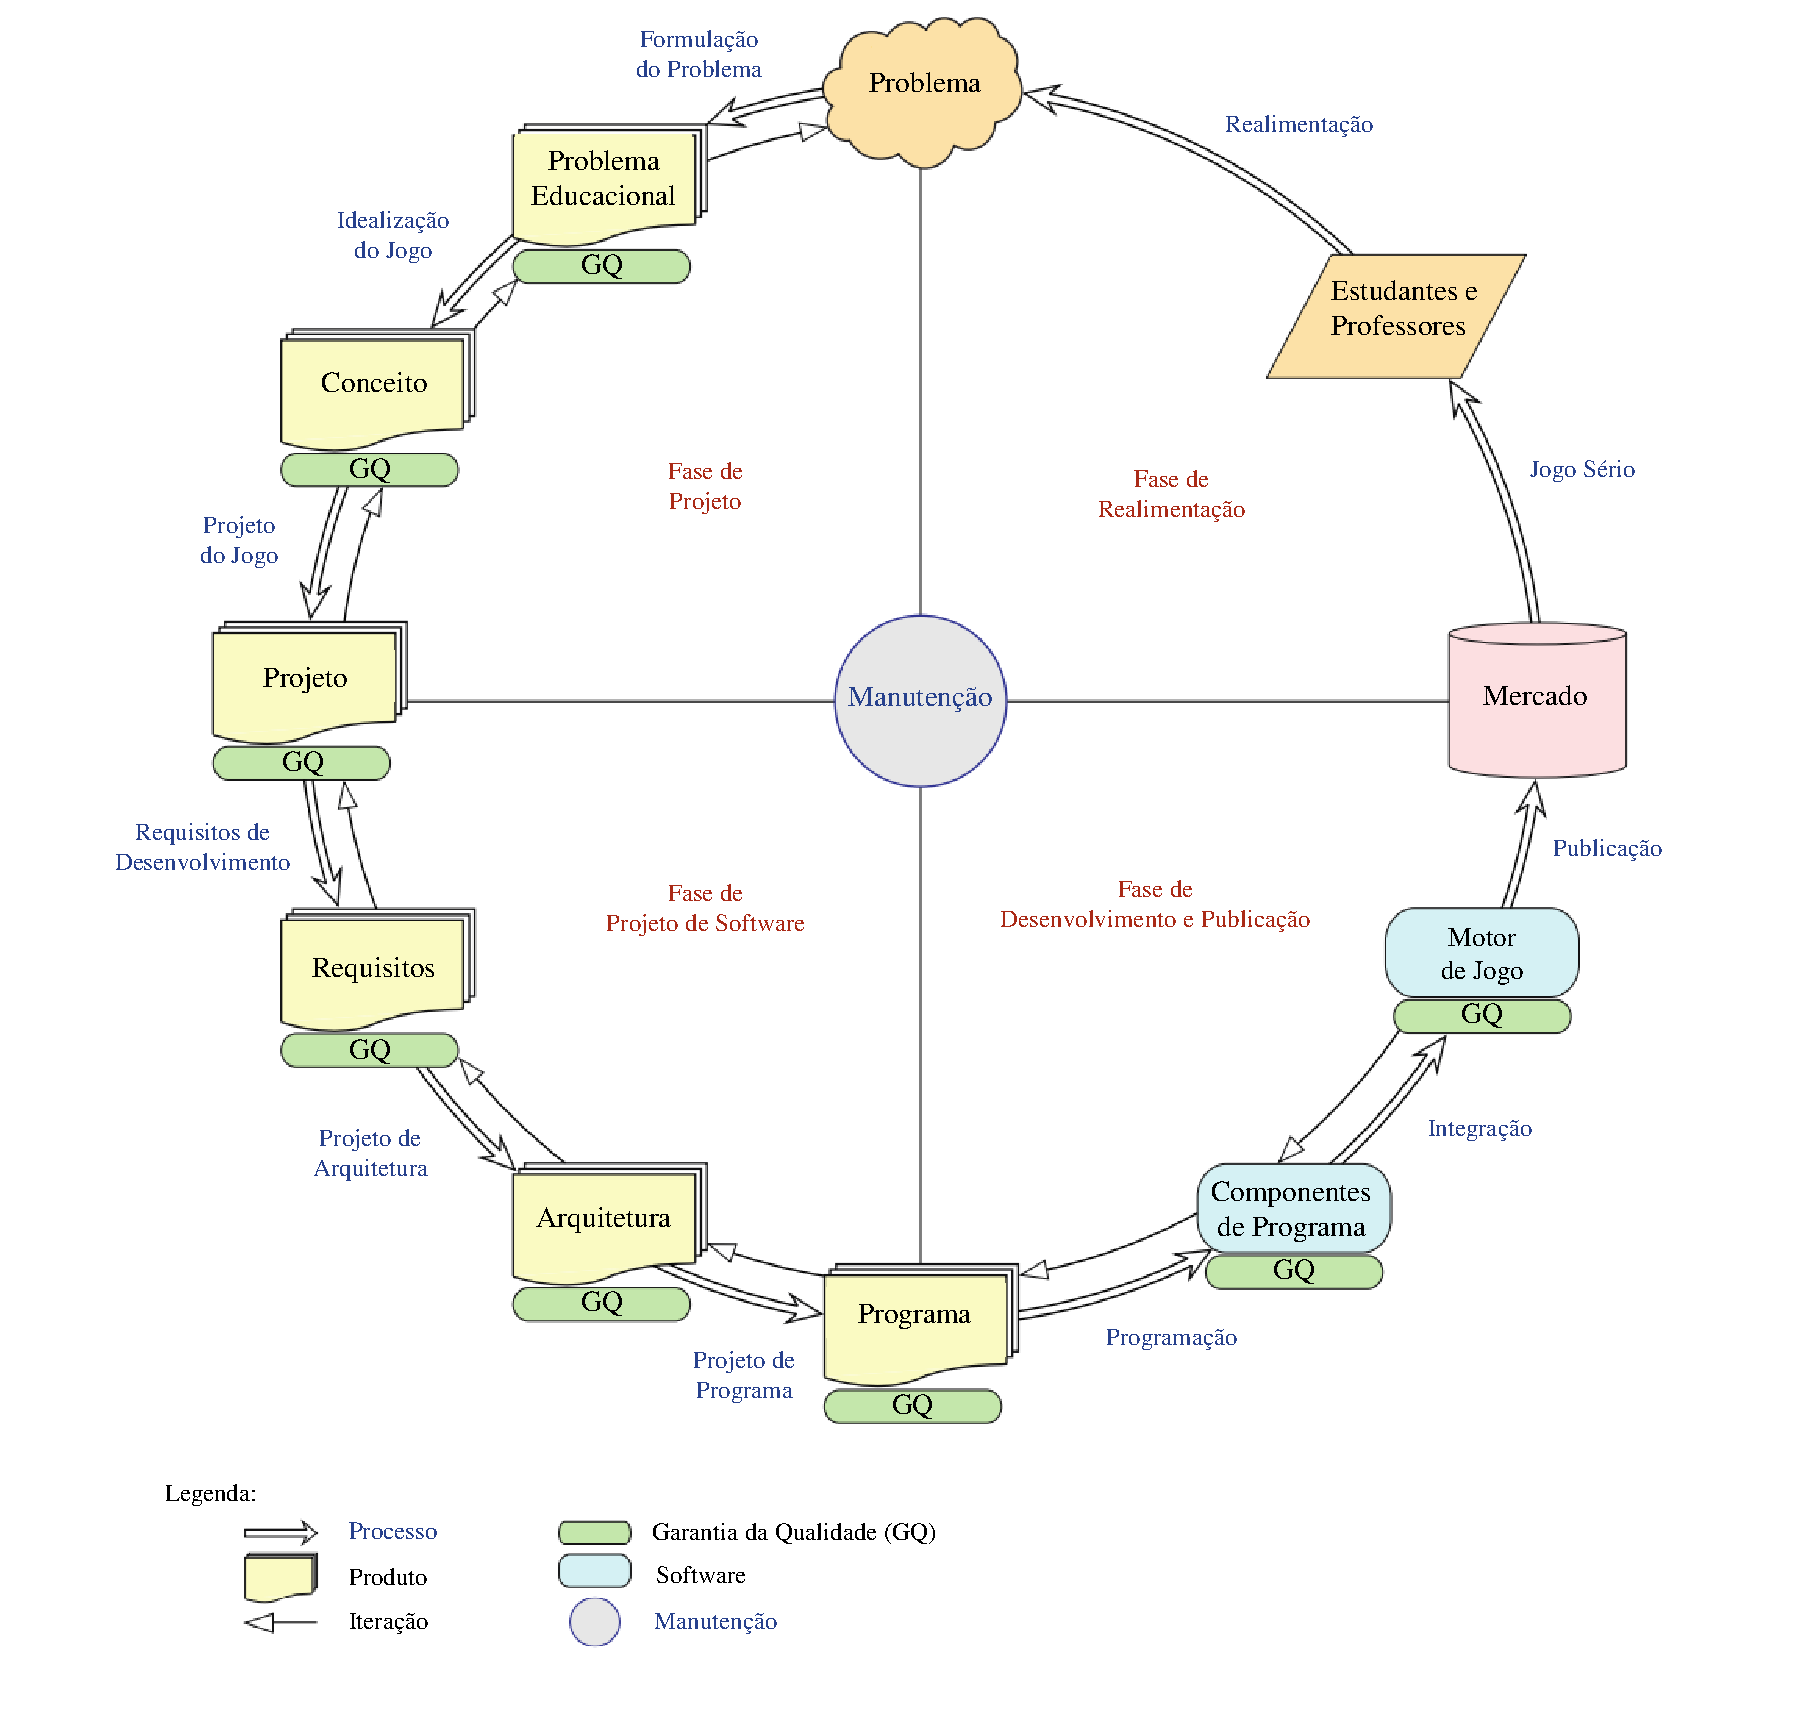
\includegraphics[width=1.05\linewidth]{./Figuras/GAMED.pdf}
	\end{center}%\vspace{-0.5cm}
  \legend{Fonte: adaptado de \cite{aslan2016digital}}

\end{figure}

O ciclo da \autoref{fig:GAMED} apresenta os processos em uma forma lógica solicitante começando de um \textbf{Problema} inicial. A partir de então o ciclo se inicia na Fase de Projeto, passando pelo Projeto de Software, pela Fase de Desenvolvimento e pela Fase de Realimentação. Ao término da última fase o ciclo se inicia novamente sendo um processo de manutenção contínuo do jogo. Cabe salientar que embora as setas mostrem um progresso sequencial, o ciclo de desenvolvimento de um jogo não precisa ser interpretado como estritamente sequencial. A representação sequencial usada na \autoref{fig:GAMED} se destina a mostrar apenas a direção do fluxo de trabalho ao longo do ciclo de desenvolvimento. 

A metodologia GAMED é iterativa tanto em sentido horário, quando em sentido anti-horário. No caso, as setas reversas almejam sanar um problema relativamente comum na área de desenvolvimento de jogos (e.g. um determinado processo pode apontar falhas no processo anterior; para arrumar a falha é recomendado retornar ao processo anterior ao invés de esperar que o ciclo se complete por inteiro). A alternância entre os processos acontece após atingir um patamar aceitável de confiança na qualidade do jogo, por tal razão cada processo passa por uma etapa de \textbf{Garantia da Qualidade (GQ)}. A qualidade só é atingida após um grupo qualificado confirmar que os seguintes conceitos estão devidamente empregados no jogo desenvolvido: Aceitabilidade, Desafio, Clareza, Eficácia, Engajamento, Diversão, Interatividade, Flexibilidade/Escalabilidade, Ludificação, Simplicidade, Aprendizagem e Usabilidade. 


%é desenvolvido somestre por um único individuo. O período de desenvolvimento está projetado para durar três meses. Os recursos necessários são programas e aparelhos já em posse do desenvolvedor. Dadas estas características a metodologia escolhida para o desenvolvimento do jogo foi a .


%Para guiar o processo de desenvolvimento de jogos, os autores apontam a divisao do ciclo de vida do jogo em 4 ˜ principais etapas, que se repetem ao longo do seu desenvolvimento, sendo elas: 1) game design; 2) game software design; 3) implementac¸ao e disponibilizac¸ ˜ ao do jogo e 4) aprendizado ˜ baseado em jogos e avaliac¸ao.

\vspace{-0.2cm}

A primeira fase do GAMED (\textbf{Fase de Projeto}) estabelece a definição de um problema no domínio educacional para ser abordado por meio da dinâmica de jogos. O atual trabalho se objetiva a fortalecer as estratégias de enfretamento ao problema da violência sexual infantil. Por tal razão, foi realizada uma formulação do problema, identificando suas causas e consequências, além da criação conceitual do jogo. Na segunda fase do GAMED (\textbf{Fase de Projeto de Software}); referente ao jogo produzido por este trabalho; foram catalogados os requisitos necessários para o desenvolvimento do jogo, além da escolha da arquitetura a ser utilizada. Um documento de requisitos é produzido nesta etapa. A terceira fase do GAMED (\textbf{Fase de Desenvolvimento/Publicação}), remete especificamente ao processo de criação e desenvolvimento do jogo. O jogo deve ser produzido nesta etapa de modo a sempre disponibilizar ao final uma versão jogável. A quarta fase do GAMED (\textbf{Fase de Realimentação}), busca apresentar um jogo brevemente finalizado a estudantes ou professores. O intuito é identificar falhas ou eventuais melhorias que podem vir a serem relatadas. Nesta etapa o jogo pode ser apresentado a outros profissionais devidamente capacitados que não precisam necessariamente contemplar o público alvo do jogo.

\vspace{-0.2cm}

O GAMED fornece um plano detalhado para o gerenciamento de projetos complexos de desenvolvimento de jogos. Sua estrutura modularizada de desenvolvimento em fases e processos facilita o desenvolvimento de jogos educacionais digitais. O GAMED ainda é flexível se adaptando as necessidades da equipe de desenvolvimento 
\cite{aslan2016digital}. Como o desenvolvimento do jogo sério deste trabalho envolveu essencialmente uma pessoa (o próprio pesquisador) algumas etapas do GAMED foram supridas a fim de agilizar o processo de desenvolvimento, porém sem perder sua essência primordial. 

\vspace{-0.2cm}

A compreensão dos fundamentos acerca o desenvolvimento de jogos educacionais digitais é indispensável para a progressão e conclusão deste trabalho. O presente trabalho baseia-se nos conceitos pesquisados e nas definições referenciadas nessa seção para fundamentar o processo de desenvolvimento.



%As metodologias de projeto instrucional são utilizadas para guiar o processo de projeto e o desenvolvimento de vários tipos de médias para a aprendizagem (McMahon, 2009). O projeto instrucional é ``a ação intencional e sistemática de ensino, que envolve o planejamento, o desenvolvimento e a utilização de métodos, técnicas, atividades, materiais, eventos e produtos educacionais em situações didáticas específicas, a fim de facilitar a aprendizagem humana a partir dos princípios de aprendizagem e instrução conhecidos'' (Filatro, 2010). O projeto de jogos sérios é um processo de exploração das teorias pedagógicas aplicadas aos jogos para criar as melhores condições de ensino e aprendizagem (Perron, 2009). Através desse processo identificam-se o que é necessário ensinar e as tarefas que o jogador necessita de completar para que a aprendizagem ocorra. Os resultados do projeto instrucional informam a equipa de desenvolvimento como apresentar a informação de uma forma que ajudará o aluno a compreendê-la (Iuppa, 2010).

%A metodologia de projeto adotado nesta investigação segue a proposta por Marfisi-Schottman et al. (2010) que constitui um modelo com sete passos, como ilustrado na Figura 4.2. Além dos passos, os autores também incluem os atores responsáveis por cada um deles. Como esta investigação envolveu essencialmente uma pessoa (o próprio investigador), foi suprimida a representação e descrição dos atores. Os modelos consideram uma equipa de desenvolvimento do jogo. Serão descritos mais simplificadamente os passos, considerando que este é um projeto de investigação envolvendo uma equipa minimalista, constituída pelo investigador e pelos seus orientadores.

%O primeiro passo é a especificação dos objetivos pedagógicos que consiste em definir o domínio de conhecimento, as capacidades e competências a serem aprendidas pelos alunos. O projetista identifica os resultados esperados na aprendizagem (memorizar, entender, aplicar, etc.) e que não devem ser confundidos com o objetivo do jogo, que é ganhar, uma vez que ganhar no jogo não está necessariamente relacionado com a aprendizagem (Van Staalduinen, 2011; Lameras et al., 2017). Nessa fase também são definidas as formas de avaliar o progresso e a aprendizagem do jogador.

%No controlo de qualidade pedagógico (sexto passo) é feita a avaliação se todos os objetivos instrucionais foram considerados (Filatro, 2008) e se a mensuração do progresso e desempenho cobrem esses objetivos (Iuppa, 2010). Deve ser feito antes do teste com utilizadores reais, e depois, como um processo de evolução constante do jogo.


%\section{Ferramentas}\label{sec:Ferramentas} FALAR EM UM PARAGRAFO NA PARTE DE DESENVOLVIMENTO


\section{Metodologia Avaliativa}\label{sec:Avaliativos}

%%%%LEEEEER: A standardised measure of child sexual abuse prevention knowledge was used: CKAQ (Tutty, 2003).
%%%%LERR: CKAQ score may be a better measure of CSA prevention knowledge between those students who complete the game and those that do not. 
%The Children's Knowledge of Abuse Questionnaire (CKAQ) is a series of statements which the child answers as being true, false or don’t know, thus demonstrating knowledge of CSA prevention but not skills. It is an ongoing challenge to measure CSA prevention skills with children, and methods typically used to assess skills in other domains such as role-play and vignettes can be less appropriate in CSA, particularly with children aged 8–10 years
%%%%%The Children's Knowledge of Abuse Questionnaire (CKAQ) does not test the likelihood to disclose and does not help us to understand why some children don’t tell. It continues to be difficult to understand why some children don’t disclose, however unlike other locations (eg some US States, Blakeya, Glaudea, & Williams Jennings, 2019),
%%%%WIST - “What if” Situation Test. = QUESTIONARIO.

%file:///C:/Users/Windows/Desktop/AQUI%20TEM%20o%20QUESTIONARIO.pdf



%Cascata = ela segue uma cascata, (1970). 5 etapa, requerimentos, design, implementação, verificação e manutenção. 

%Espiral (1986) = ciclos iterativos, criação de prototipos. [AVALIAÇÃO DE RISCO] mais felivel e evita o retrabalho. 

%Evolutiva = prototipo inicial que vai evoluindo. 

%Scrum = dá a possibilidade de já ter um produto funcional (mesmo sem estar completo) [equipes pequenas  + equipes com perfil interdisciplinar] o que foi feito? o que será feito ainda? quais suas dificuldades?

%XP = eXtreme Programming [pessoas mistruram com a Scrum e usam o XP especifico para o desenvolvimento de jogos (programação)]

% as metodologias ágeis não são tão rídigas, proprocionam um desenvolvimento ágil que pode se adaptar a adversidades encontradas durante o desenvolvimento. 

%%%%%%%O ensino de desenvolvimento de jogos é uma tarefa não-trivial, por se tratar de uma categoria de software com um conjunto de requisitos bastante específicos e demandas tecnológicas singulares. O uso de metodologias ágeis para o desenvolvimento de jogos pode facilitar esse processo de desenvolvimento e conseqüentemente influenciar na aprendizagem desse processo.


%%%%%%%%%%%5) Game Design Document (GDD) [25]: É um documento guia do processo de desenvolvimento de um jogo e é dependente do contexto de cada projeto. O GDD precisa conter detalhes de jogabilidade, enredo, personagens, interface e regras do jogo. A falta dele pode ocasionar problemas sérios de design, falta de recursos e dificuldades de corrigir eventuais problemas [16]. %http://sbgames.org/sbgames2018/files/papers/ArtesDesignFull/188093.pdf


%1) Metodologia Maiêutica (M2 ) [22]: Apresenta uma proposta de metodologia de desenvolvimento de Ambientes Virtuais 3D Interativos com foco no processo de ensino e aprendizagem. O diferencial desta metodologia é a forma como ela conduz o processo de concepção, induzindo a reflexão e a criatividade.%http://sbgames.org/sbgames2018/files/papers/ArtesDesignFull/188093.pdf


%Assim, guias ou metodologias de desenvolvimento de jogos podem servir de base para a construção de games. Todavia, recente pesquisa \cite{buchinger2013jogos} indicou que não existe uma metodologia sólida para a construção de JSCC.




%Avaliar a aprendizagem exige uma abordagem sistemática para determinar o sucesso e as dificuldades dos alunos (Bellotti et al., 2013). O grande desafio para criar essas avaliações é que necessitam naturalmente de serem tarefas do jogo, onde não se sacrifique a confiabilidade e validade do processo (Shute & Ke, 2012) e não se interrompa o fluxo na experiência de jogo correndo o risco do aluno perder o interesse (Chen, 2007). As interações com o jogo, ou seja, a sequência das ações, é que demonstram, com base nas escolhas do aluno, o que sabe ou não do assunto. O progresso do aluno ao avançar num jogo e acumular pontos de experiência pode ser uma evidência da sua aprendizagem. Não conseguir superar os desafios do jogo, representa que o aluno tem deficiências quanto às competências necessárias para fazê-lo, e rastrear as suas tentativas pode apontar quais são esses problemas e o apoio que necessita. Essas interações geram usualmente uma grande quantidade de dados a serem analisados. [tese ADILSON]

%https://sci-hub.se/https://doi.org/10.1016/0145-2134(94)90119-8
%https://watermark.silverchair.com/19-2-112.pdf?token=AQECAHi208BE49Ooan9kkhW_Ercy7Dm3ZL_9Cf3qfKAc485ysgAAAqAwggKcBgkqhkiG9w0BBwagggKNMIICiQIBADCCAoIGCSqGSIb3DQEHATAeBglghkgBZQMEAS4wEQQMb7ij4AZzJ8owkcuvAgEQgIICU_1hK9OxMHlS85hxu2mBEgwar_CU1oIQAD8Nybb296oxklF-bIuCo1ObyypZLxrOuopvv5a7e10N5dTZWrxD0LI05SPlWKLaEypJbQ-rffskRKQWXtFhevnphnPLJUfIFAjJ6nBps88dphBtn1YMkptIBJsbokecwixvaD6ULoOth9O9sxsqttPmfNDEJbf3aN9IiyuXMfb18yU8Wx57fGR6zjBrOSE7NHGSJTKzJj8SV0SKEI6i8MX2cxk2mY3TrZG8FI3KT1VZITx1iBW3vwpLrH0d6ISVwBniQ54PfHNYXiuAzQ1S_TSdjV4-eUbxkRs9jbOtzb0C5KwzROmAUMk-MEBQRPjLLJrDZwj7CN1o5shEliVoG42hDw--jZA6Zp6OIirgrtfXHYEtiHnhC4lXg5cyrKQJyeXrnuU0714YCnhwGCq3tAMckt9uo8Ybp7egsmVqJJvYQ_jjTfr984-IsG329I4Pi8i1Rlf3xlXLGiA8htPh3TIe8MnqRT0uQonYnT6_Biz2KoezhHq3BQFsRbnMgJbqppmDT0L_5-TJMDhU_FTleD66n5w-vmBDyvtrHi6NwaROedYhj-6RkdE_04lsCzzkk7H3hWgmIb7-FCVqaTo0LS1vrPEuxvsgEtjVN6J4J_On1GbUpGHnk4E6wEVfDxmt8SVnSAhpEASOlUDG8Rk95ZZK1h1hUo1g3rJKWMrTuwTE1EhVBX-imJWj0WHmvFxXCsOLV4yFREXnngAbSiMsW_lbzpSXdSgghKDT6h9eau5XBKpgSoBRWCqQv1I = The revised Children's Knowledge of Abuse Questionnaire: Development of a measure of children's understanding of sexual abuse prevention concepts
%https://sci-hub.se/10.1016/0145-2134(92)90046-T
%https://sci-hub.se/https://doi.org/10.1080/10538712.2019.1688443


A avaliação de jogos é utilizada para medir o nível de sucesso de uma solução educacional, ou seja, se ela possibilita alcançar os objetivos que foram estabelecidos. Existem inúmeros métodos e modelos para avaliação de jogos no contexto educacional, no entanto, a maioria das soluções avaliativas oferecidas as crianças no ensino fundamental, não estão amplamente disponíveis \cite{tutty2019children}. A literatura relata alguns jogos voltados para a prevenção da violência sexual infantil (\autoref{ch:Relacionados}). Dentre os jogos voltados para essa temática o modelo avaliativo mais utilizado é o \textit{Children’s Knowledge of Abuse Questionnaire} - (CKAQ)% Questionário Sobre Conhecimentos de Abuso Infantil (em inglês: \textit{Children’s Knowledge of Abuse Questionnaire} - CKAQ).

\vspace{-0.1cm}

O \textit{Children’s Knowledge of Abuse Questionnaire} é um questionário desenvolvido para avaliar os níveis de conhecimento dos conceitos de prevenção de abuso para crianças em idade de cinco a doze anos \cite{tutty1992ability}. No caso das crianças mais novas se recomenda que o questionário seja administrado verbalmente e de modo individual, caso seja observado níveis incompletos de alfabetização e leitura. O questionário é constituído por questões de múltipla escolha (verdadeiro/falso).

\vspace{-0.1cm}

O questionário em questão possui algumas versões que foram produzidas ao longo dos anos \cite{tutty1995revised, tutty2019children}. No geral as versões variam apenas em números de questões, existindo versões do questionário com apenas dez questões, construídas com o intuito de auxiliar o pesquisador e agilizar os experimentos. Os questionários resumidos apresentam um grau de confiança aceitável para pesquisas, contudo são aconselháveis apenas para as situações nas quais a medição dos conhecimentos sobre a prevenção da violência infantil não sejam o foco da pesquisa. 

%O questionario revisado de 24 itens era composto pela subescala Toque Inadequado (Mau)

%no questionário original, a pontuação é feita em 0 e 1.

\vspace{-0.1cm}

A versão revisada do questionário (\autoref{chap:CKAQ}), composto por 33 questões, apresenta largo uso nas pesquisas e demonstra-se apropriado ao avaliar o conhecimento aprofundado dos conceitos básicos de prevenção incluídos em programas de educação de prevenção ao abuso sexual infantil \cite{tutty1992ability}. O presente trabalho traduziu para o português o CKAQ original (\autoref{chap:traduzido})). A versão traduzida do questionário é utilizada pelo presente trabalho para validar o programa educacional proposto pela atual pesquisa, o processo de validação é melhor descrito na \autoref{ch:Avaliacao}.

%The Children’s Knowledge of Abuse Questionnaire (CKAQ) and versions thereof (CKAQ-R, CKAQ-IIIR) were used in five studies

% escala não possui pontos de corte, mas escores mais altos indicam maior conhecimento sobre prevenção do abuso sexual. 

%A pontuação a ser obtida neste questionário varia entre 0 e 33, e pontuações mais altas indicam mais conhecimento sobre a prevenção do abuso sexua

\vspace{-0.1cm}

A compreensão dos fundamentos para a validação de jogos educacionais é indispensável para a progressão e conclusão deste trabalho. O presente trabalho baseia-se nos conceitos pesquisados e nas definições referenciadas nessa seção para fundamentar e guiar o processo de validação do jogo desenvolvido por esta pesquisa. A validação e submissão do questionário ocorre em dois momentos distintos da pesquisa, na etapa de pré-teste e pós-teste. Para o processo avaliativo utilizou-se dois grupos, um grupo experimental e um grupo controle sem quaisquer diferenças étnicas ou socie-econômicas aparentes entre os grupos (e dentro dos grupos). Para a comparação dos resultados entre os grupos utilizou-se o Teste-t. 

%POR NÃO TER MUITAS DIFERENÇAS ETNICAS OU SOCIO-ECONOMICAS A AMOSTRA NÃO É ALEATORIO, POR ISSO ESSA É UMA PESQUISA QUASE-EXPERIMENTAL. 

%FORAM COLETADOS OS DESEMPENHOS OS GRUPOS VIA REDE, OS ACERTO E ERROS ERAM ANEXADO EM UM BANCO DE DADOS RELACIONAL A FIM DE COMPARAR COM OS RESULTADOS DOS TESTES (NO CASO DO GRUPO EXPERIMENTAL). ASSIM, É POSSIVEL OBSERVAR UMA POSSIVEL RELAÇÃO ENTRE O DESEMENHO NO JOGO E NAS APRENDIZAGEM ADQUIRIDAS PELO JOGADOR (OU NÃO).

%Os níveis de conhecimento dos conceitos de prevenção de abuso foram testados usando o Children's Knowledge of Abuse Questionnaire-Revised (CKAQ-R), uma medida padronizada que foi desenvolvida para crianças em idade escolar do primeiro ao sexto ano. O CKAQ-R usa um formato verdadeiro-falso e tem fortes propriedades psicométricas

\begin{comment}

%das estratégias de avaliação utilizadas como base para o modelo desenvolvido por \citeonline{savi2011avaliaccao}. Em aspectos estruturais a \autoref{Kirkpatrick} apresenta o modelo de Kirkpatrick, a \autoref{ARCS} apresenta o modelo \ac{ARCS}, a \autoref{EEUU} apresenta conceitos de experiência do usuário, a s\autoref{Bloom} apresenta a taxonomia de Bloom, e por fim, a \autoref{savizinho} apresenta o modelo teórico de avaliação desenvolvido por \citeonline{savi2011avaliaccao}.

\subsection{Kirkpatrick}
\label{Kirkpatrick}

Donald Kirkpatrick criou o método de avaliação de treinamento baseado em quatro diferentes níveis: reação, aprendizagem, comportamento e resultados \cite{donald1994evaluating}. Cada nível tem sua importância e, conforme se passa de um nível para outro seguinte, o processo se torna mais complexo e demorado, porém fornece resultados mais valiosos \cite{chapman2009kirkpatrick}. Em linhas gerais, a definição de cada um dos níveis pode ser feita da seguinte maneira:


\begin{itemize}[label={},leftmargin=2em]
\item \textbf{Reação}: Avalia a experiência de aprendizagem a partir da percepção dos participantes. Para isso, utiliza como ferramenta de avaliação formulários de \textit{feedback}, pesquisas após o treinamento ou questionários.
\end{itemize}



\begin{itemize}[label={},leftmargin=2em]
\item \textbf{Aprendizagem}: Avalia o aumento de conhecimento, utilizando-se de avaliações e testes, além de entrevistas ou observações.
\end{itemize}

\begin{itemize}[label={},leftmargin=2em]
\item \textbf{Comportamento}: Avalia os efeitos da nova aprendizagem por meio de observações ou entrevistas ao longo do tempo. Desta forma, busca-se avaliar as mudanças comportamentais, avaliar a relevância das mudanças e avaliar a sustentabilidade das mudanças. 
\end{itemize}

\begin{itemize}[label={},leftmargin=2em]
\item \textbf{Resultados}: Avaliam os efeitos do treinamento do aluno. Para isso, utiliza de ferramentas como questionários, observações ou entrevistas.
\end{itemize}


\pagebreak

\subsection{ARCS}
\label{ARCS}

O modelo \ac{ARCS} tem como objetivo principal empregar estratégias motivacionais no projeto de materiais educacionais \cite{keller1983development}. Este modelo foca na interação dos alunos com os materiais e ambientes de aprendizagem e é derivado da teoria expectativa-valor. Tal teoria aponta que a expectativa (que está ligada a uma probabilidade subjetiva de um indivíduo obter sucesso) e valores (que estão ligados a satisfação de necessidades pessoais ou motivos) são determinantes chave do esforço empregado em uma atividade. 

O nome do modelo é um acrônimo para: Atenção, Relevância, Confiança, Satisfação. Cada um dos termos que compõem o nome do modelo são peças fundamentais para a sua formulação \cite{keller1983development}. Suas definições seguem da seguinte maneira: 

\begin{itemize}[label={},leftmargin=2em]
\item \textbf{Atenção}: Refere-se às respostas cognitivas dos alunos aos estímulos instrucionais. A atenção é um elemento motivacional e pré-requisito para a aprendizagem. O desafio é obter e manter um nível satisfatório da atenção dos alunos ao longo de um período de aprendizagem.
\end{itemize} 

\begin{itemize}[label={},leftmargin=2em]
\item \textbf{Relevância}: A relevância se preocupa em garantir que uma proposta educacional seja consistente a ponto de conseguir conectar o conteúdo da aprendizagem com sua aplicação em cenários reais. A relevância também quantifica as associações que os alunos conseguem fazer entre seus conhecimentos prévios e as novas informações.
\end{itemize}

\begin{itemize}[label={},leftmargin=2em]
\item \textbf{Confiança}: Está relacionada com a criação de expectativas positivas aos estudantes. Isso pode ser alcançado ao se proporcionar experiências de sucesso no uso do material escolar decorrentes da própria habilidade e esforço dos alunos. Este fator tem influência na persistência dos estudantes.
\end{itemize}

\begin{itemize}[label={},leftmargin=2em]
\item \textbf{Satisfação}: Os alunos precisam ter sentimentos positivos sobre a experiência de aprendizagem, e isso pode vir com recompensas e reconhecimento. Também recomenda-se providenciar tão cedo quanto possível oportunidades para os alunos aplicarem o que foi aprendido. Os estudantes devem sentir que o esforço dedicado aos estudos foi apropriado e que houve consistência entre objetivos, conteúdo e testes de avaliações.
\end{itemize}

\pagebreak


\subsection{Experiência do Usuário}
\label{EEUU}

A \ac{UX} (em português, \textbf{experiência do usuário}) analisa a percepção e resposta de uma pessoa sobre o uso de um produto, sistema ou serviço. Os produtos, ao invés de serem vistos como um pacote de funcionalidades e benefícios, são vistos como um gerador de experiências. Essas experiências, decorrentes da interação, podem gerar mudanças no estado emocional das pessoas \cite{calvillo2009core}, e é objetivo da \ac{UX} avaliar e ampliar o entendimento das experiências que as pessoas têm com os produtos.

\citeonline{savi2011avaliaccao} destaca quatro modelos, usados para mensurar a experiência do usuário: \citeonline{takatalo2010presence, poels2007always, calvillo2009core, sweetser2005gameflow}. Tais modelos são apresentados em maiores detalhes no anexo deste trabalho, respectivamente: \autoref{chap:A5}, \ref{chap:A6}, \ref{chap:A7}, \ref{chap:A8}. Em linhas gerais, os conceitos fundamentais desses quatro modelos adotados por \citeonline{savi2011avaliaccao} são: 

\begin{itemize}[label={},leftmargin=2em]
\item \textbf{Imersão}: Mensura a distorção da noção temporal dos jogadores, relacionada com a experiência de profundo envolvimento no jogo, levando em consideração o desvio de foco do mundo real para o mundo do jogo.
\end{itemize}

\begin{itemize}[label={},leftmargin=2em]
\item \textbf{Interação Social}: Mede a conexão de um jogador com demais jogadores, em termos de cooperação, conquistas e união. O envolvimento do usuário com outras pessoas é um elemento de diversão usado para medir a experiência do jogador nesse aspecto. 
\end{itemize}

\begin{itemize}[label={},leftmargin=2em]
\item \textbf{Desafio}: É responsável pela compreensão da satisfação do usuário em relação ao nível de dificuldade, devendo existir um equilíbrio que agrade o jogador.
\end{itemize}

\begin{itemize}[label={},leftmargin=2em]
\item \textbf{Divertimento}: Mensura de modo geral os sentimentos de diversão, prazer, relaxamento, distração e satisfação; sendo levado em consideração o interesse do jogador em voltar a jogar ou recomendar o jogo.
\end{itemize}

\begin{itemize}[label={},leftmargin=2em]
\item \textbf{Controle}: Quantifica a sensação de independência, poder e liberdade do jogador no jogo. Compreende em linhas gerais, a bijeção entre as ações do jogador e as respostas do personagem do jogador no jogo. 
\end{itemize}

\begin{itemize}[label={},leftmargin=2em]
\item \textbf{Competência}: A competência é uma medida combinada de habilidades do jogador e sentimentos positivos de eficiência. Está relacionada com a percepção de habilidades, controle e uso dessas habilidades para explorar o jogo e progredir.
\end{itemize}




\subsection{Taxonomia de Bloom}
\label{Bloom}

A taxonomia de Bloom foi criada com o objetivo de apoiar os processos de projeto e avaliação educacional, podendo ser aplicada para planejar, projetar e avaliar a efetividade da aprendizagem e de treinamentos \cite{bloom1956taxonomy}. A taxonomia de Bloom tem uma proposta que abrange e aborda tanto o domínio motor, quanto o domínio cognitivo \cite{moody2003evaluating}. Sua estrutura está definida em seis níveis:

\begin{itemize}[label={},leftmargin=2em]
\item \textbf{Conhecimento}: Habilidade de lembrar informações e conteúdos previamente abordados como fatos, datas, palavras, teorias, métodos, classificações, lugares, regras, critérios, procedimentos, etc. A habilidade pode envolver lembrar uma significativa quantidade de informação ou fatos específicos.
\end{itemize}
\vspace{-0.4cm}
\begin{itemize}[label={},leftmargin=2em]
\item \textbf{Compreensão}: Habilidade de compreender e dar significado ao conteúdo. Essa habilidade pode ser demonstrada por meio da tradução do conteúdo compreendido para uma nova forma contextual, oral ou escrita. Nessa categoria, encontra-se a capacidade de entender a informação ou fato, de captar seu significado e de utilizá-la em contextos diferentes.
\end{itemize}
\vspace{-0.4cm}
\begin{itemize}[label={},leftmargin=2em]
\item \textbf{Aplicação}: Habilidade de usar informações, métodos e conteúdos aprendidos em novas situações concretas. Isso pode incluir aplicações de regras, métodos, modelos, conceitos, princípios, leis e teorias. 
\end{itemize}
\vspace{-0.4cm}
\begin{itemize}[label={},leftmargin=2em]
\item \textbf{Análise}: Habilidade de subdividir o conteúdo em partes menores com a finalidade de entender a estrutura final. Essa habilidade pode incluir a identificação das partes, análise de relacionamento entre as partes e reconhecimento dos princípios organizacionais envolvidos. Nesse ponto é necessário não apenas ter compreendido o conteúdo, mas também a estrutura do objeto de estudo, identificando suas partes e suas inter-relações.
\end{itemize}
\vspace{-0.4cm}
\begin{itemize}[label={},leftmargin=2em]
\item \textbf{Síntese}: Habilidade de agregar e juntar partes com a finalidade de criar um novo todo. Essa habilidade envolve a produção de uma comunicação única (tema ou discurso), um plano de operações (propostas de pesquisas) ou um conjunto de relações abstratas (esquema para classificar informações). 
\end{itemize}
\vspace{-0.4cm}
\begin{itemize}[label={},leftmargin=2em]
\item \textbf{Avaliação}: Habilidade de julgar o valor do material para um propósito específico. O julgamento é baseado em critérios bem definidos que podem ser externos (relevância) ou internos (organização) e podem ser fornecidos ou conjuntamente identificados.
\end{itemize}


\subsection{Modelo teórico de Savi}
\label{savizinho}

\citeonline{savi2011avaliaccao} desenvolveu um modelo para a avaliação da qualidade de jogos educacionais baseado no modelo de avaliação de treinamentos de Kirkpatrick (\autoref{Kirkpatrick}), nas estratégias motivacionais do modelo ARCS (\autoref{ARCS}), na área de experiência do usuário (\autoref{EEUU}) e na taxonomia de objetivos educacionais de Bloom (\autoref{Bloom}). O modelo de \citeonline{savi2011avaliaccao} se destoa dos demais por proporcionar um aumento na confiabilidade das avaliações de jogos educacionais \cite{savi2010proposta}. Além disso, o modelo em questão demanda baixo esforço de customização e pode ser aplicado tanto em jogos de tabuleiro, quanto em jogos digitais. 

O modelo de \citeonline{savi2011avaliaccao} agregou teorias da área de design instrucional e educação. A união dos estudos de \ac{UX}, do modelo \ac{ARCS}, da taxonomia de Bloom, do modelo de Kirkpatrick culminaram em um instrumento medidor da qualidade de jogos educacionais composto por três subcomponentes: motivação, experiência do usuário e aprendizagem. Cada método (\ac{UX}, Kirkpatrick, Bloom, \ac{ARCS}) contribuiu de forma distinta para a formulação do modelo teórico de \citeonline{savi2011avaliaccao}.

Para a fundamentação do modelo de \citeonline{savi2011avaliaccao}, a área de experiência do usuário é inteiramente usada (levando em consideração a subseção \ref{EEUU} apenas). Em contrapartida apenas o primeiro nível (\textbf{reação}) do método de Kirkpatrick é usado. O modelo \ac{ARCS} contribui com seus quatro níveis (\textbf{atenção}, \textbf{relevância}, \textbf{confiança} e \textbf{satisfação}). E a taxonomia de Bloom contribui somente com os seus três primeiros níveis (\textbf{conhecimento}, \textbf{compreensão} e \textbf{aplicação}). A fundamentação da escolha de tais níveis é descrita em maiores detalhes no artigo original de \citeonline{savi2011avaliaccao}. A estrutura do modelo em questão se faz presente na \autoref{fig:saaviw}.


%figura estava aqui



A estrutura do modelo teórico de \citeonline{savi2011avaliaccao} é mostrada na  \autoref{fig:saaviw}. Nela os círculos representam os constructos teóricos do modelo, ou seja, as variáveis latentes, e os retângulos representam as dimensões que compõem as variáveis latentes. O círculo mais à esquerda representa a variável latente \textbf{reação} (reação dos alunos ao jogo educacional, como proposto por Kirkpatrick). O círculo superior compreende conceitos do modelo ARCS para avaliação do nível de \textbf{motivação}. O círculo mais ao centro aborda componentes sobre a \textbf{experiência dos usuários}. E o círculo inferior traz princípios da taxonomia de Bloom para avaliar a percepção educacional dos usuários e seu \textbf{conhecimento}. Cada círculo se ramifica em retângulos, cada qual, abordando conceitos de seus modelos base. 

\pagebreak

\begin{figure}[h]
	\centering
	\caption{Modelo de Avaliação de Jogos Educacionais}
	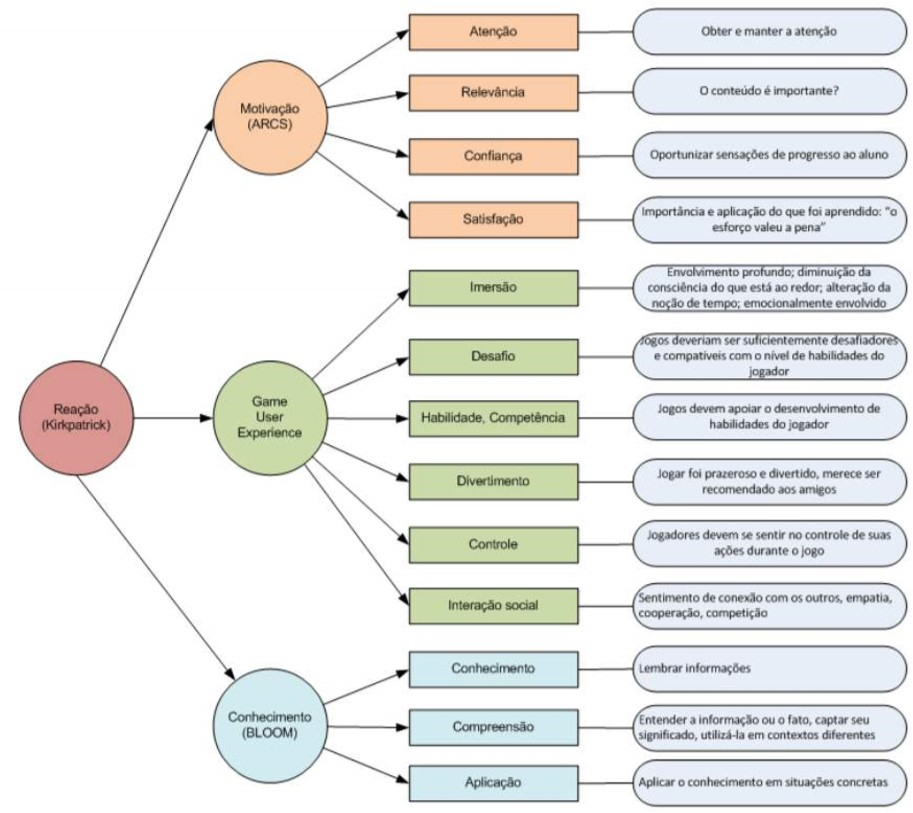
\includegraphics[width=1.0\textwidth]{Figuras/Savi.jpg}
	\label{fig:saaviw}\\
	Fonte: \citeonline{savi2011avaliaccao}.
\end{figure}
%\vspace{-0.8cm}


Os constructos do modelo teórico para avaliação de jogos educacionais desenvolvido por \citeonline{savi2011avaliaccao} são medidos por meio de itens de um questionário que foi concebido por um misto de itens padronizados e itens customizados para a avaliação da aprendizagem. Os questionários, planilhas e demais materiais referentes ao trabalho de \citeonline{savi2011avaliaccao} podem ser encontrados tanto em seu \textit{website}\footnote{\url{https://sites.google.com/site/avaliacaodejogoseducacionais}} quanto no apêndice da presente pesquisa (\autoref{chap:A1}).

\newpage

%\section{Learning Analytics}\label{sec:LA}

\end{comment}